\section{MCTuning}
\label{sec:MCTuning}

%-------------------------------------------------------------------------------
In this section we describe how the Monte Carlo samples have been 
tuned and cross-checked against data. The tuning procedure is two-fold: 
a first set of weights ("Quark Level Corrections" or QLC) accounts for 
the ($pT_B$, $\eta_B$) selection bias introduced to expedite the MC 
generation of $b$ quarks; a second set of weights ("Data Driven 
Weights" or DDW) accounts for  residual data-MC ($pT_B$, $\eta_B$) discrepancies.\\
All MC samples will be consistently used across these studies 
after applying both sets of complementary corrections: Quark 
Level and Data Driven, which are meant to be used in combination in 
order to obtain meaningful responses from the MC, with a clear 
way of accounting for residual discrepancies through systematic uncertainties.

\subsection{Quark Level Corrections}
\label{subsec:QLC}
In order to enhance the MC production efficiency the default 
MCs are generated with relatively tight parameters of the quark-level 
process and with a selection applied to the particles in the final 
state. Quark Level Corrections (QLC) are intended to correct 
and evaluate the systematics uncertainty due to the quark-level cuts, 
while effects due to the cuts on the final state 
particles are included in the analysis efficiency and acceptance studies.\\
The QLC are evaluated using two different MC samples, % (\textit{unbiased} MC and \textit{quark biased} MC), 
generated with looser quark-level cuts with respect to the default MC 
and no cuts on the final state particles ((\textit{unbiased} MC), and 
with the same quark-level cuts as the default MCs and without 
final state particle cuts (\textit{quark biased} MC).
Since QLC are meant to correct generator-level biases, 
the production of the unbiased and quark biased MCs is limited to 
generation, without simulation of the detector response and reconstruction; 
table \ref{table:genCuts} shows the sets of cuts applied at generation level for the different MCs.\\
\begin{table}[h]
  \begin{center} 
    \begin{tabular}{| c | c | c | c | c | c | c | c |}
      \hline
      & $\hat{pT}min$ &  anti-b $\eta$  &  anti-b pT  &  muons  $\eta$  &   muons pT  & final h  $\eta$  &  final h pT \\ \hline
      default $B^+ \to J/\psi K^+$  & 7 GeV &  2.6  &  7 GeV  &  2.6  &   3.5 GeV  & 2.6  & 900 MeV \\ \hline
      unbiased $B^+ \to J/\psi K^+$  & 5 GeV &  4  &  2.5 GeV  &   &    &  &  \\ \hline
      quark biased $B^+ \to J/\psi K^+$  & 7 GeV &  2.6  &  7 GeV  &    &    &  & \\ \hline
      default $B_s \to \mu^+ \mu^-$  & 5 GeV  &  2.6  & 5 GeV  &  2.6  &  3.5 GeV   &  &  \\ \hline
      unbiased $B_s \to \mu^+ \mu^-$  & 5 GeV  &  4  & 2.5  &    &     &  &  \\ \hline
      quark biased $B_s \to \mu^+ \mu^-$  &  5 GeV & 2.6   &  5 GeV &    &     &  &  \\ \hline
      default $B-s \to J/\psi \phi$  & 11 GeV  &  2.5  & 9 GeV  &  2.6  &  3.5 GeV   &  2.6 &  0.8 GeV \\ \hline
      unbiased $B-s \to J/\psi \phi$  & 5 GeV  & 4   & 2.5 GeV  &    &     &  &  \\ \hline
      quark biased $B-s \to J/\psi \phi$  &  11 GeV &  2.5  & 9 GeV  &    &     &  &  \\ \hline
    \end{tabular}
    \caption{Quark-level and final state particle cuts per MC sample.}
    \label{table:genCuts}  
  \end{center}
\end{table}

%%%%%%%old considerations about pTHat issue, might go into an appendix
%\yel[Historical perspective may not be the best way of discussing this and risks to emphasize Run 1 analysis issues rather than the point to be made]{At first QLC have been evaluated} in a similar way as in previous versions of the analysis \cite{Alpigiani:1756291}, according to the following formula:
%$$W_{QL} = \frac{\nu^{unbiased+QLsel+FScuts}(pT_B, \eta_B)}{\nu^{unbiased+FScuts}(pT_B, \eta_B)}$$
%Where $\nu$ is the number of entries in a ($pT_B$, $\eta_B$) bin and the quark-level selection (QLsel) and final state particle cuts ( FScuts), implicit in the default MC sample, are explicitly applied to the unbiased sample. The inverse of such efficiencies should be used to weight events individually, thus correcting with event-weights the QL cut biases.\\
%\begin{figure}[h]
%  \centering
%  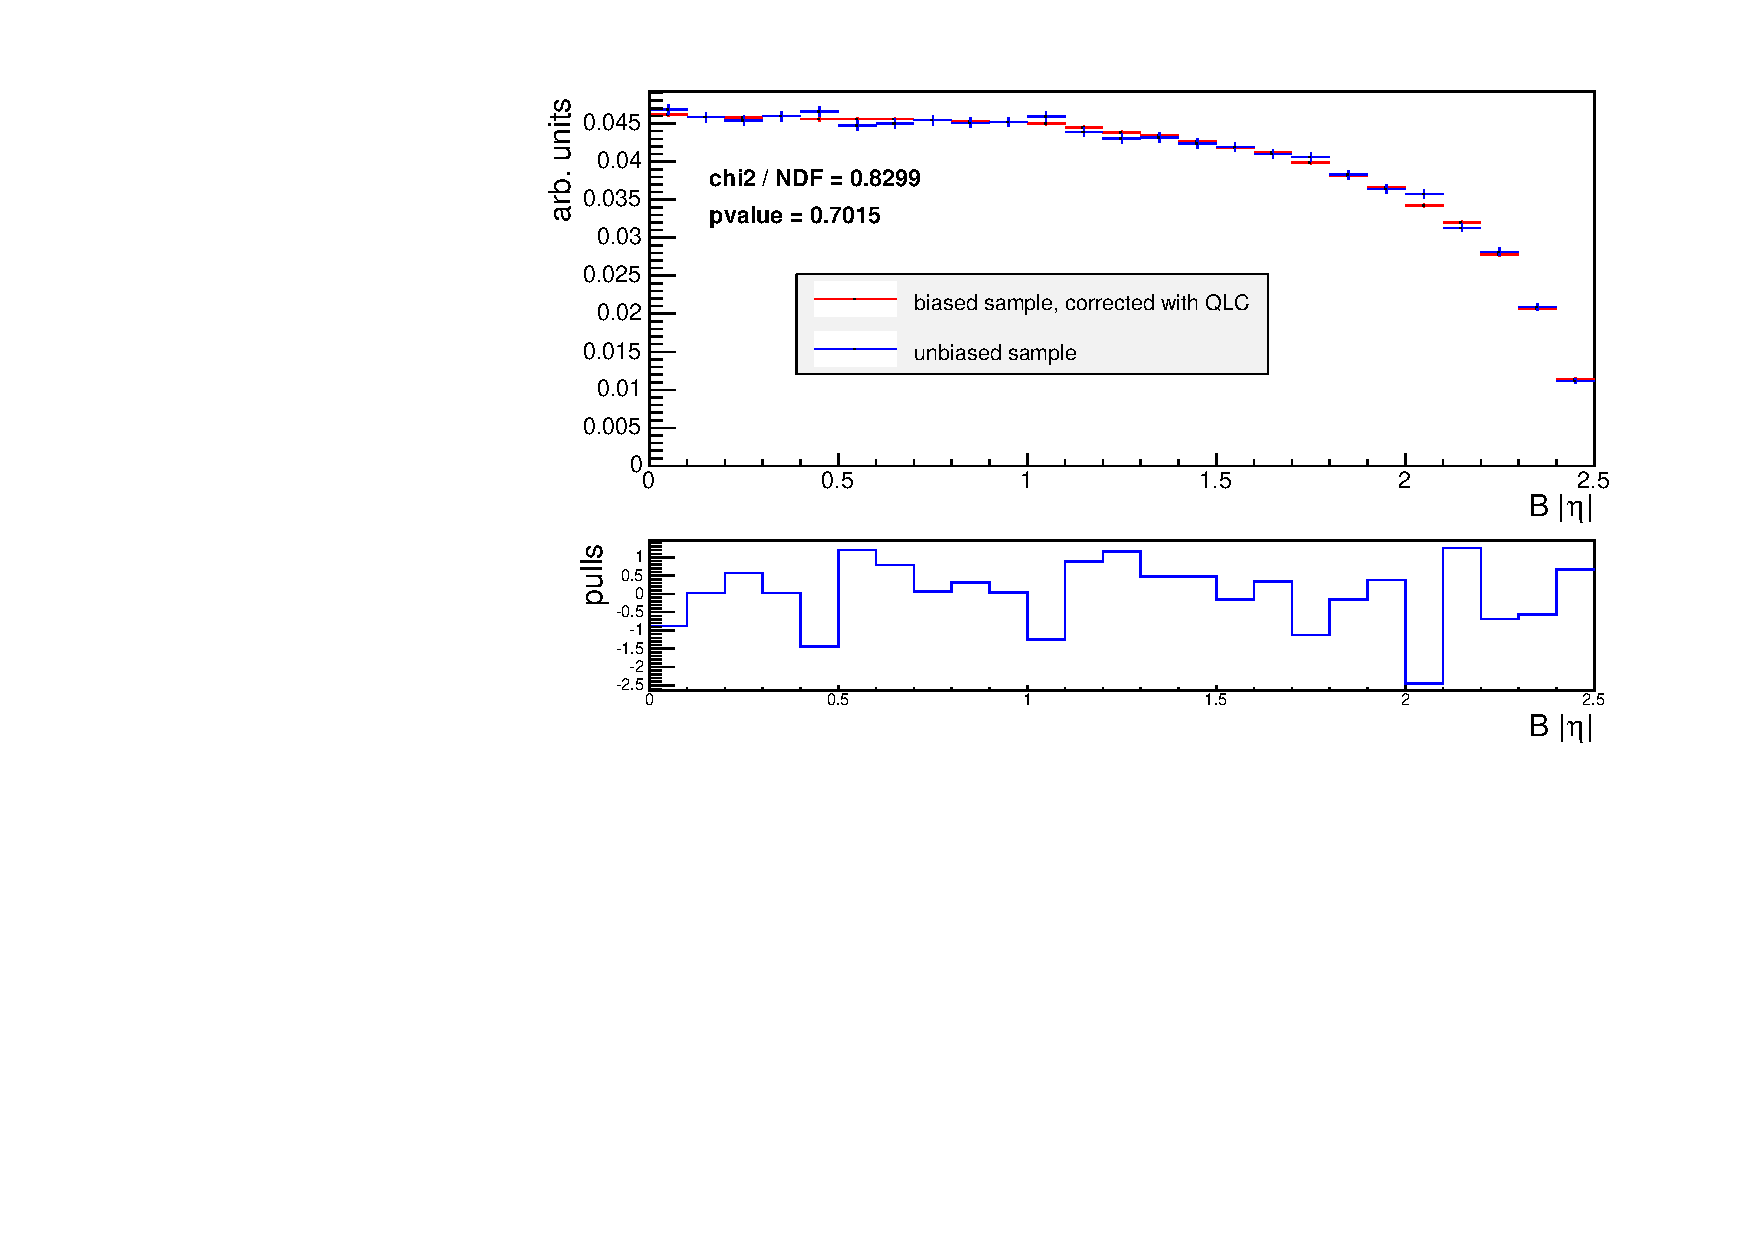
\includegraphics[width=15cm]{figures/InternalNote_MCTuning/oneSample_unbiasedVsQuarkBiasedComparison_eta.pdf}\\
%  \vspace{0.5cm}
%  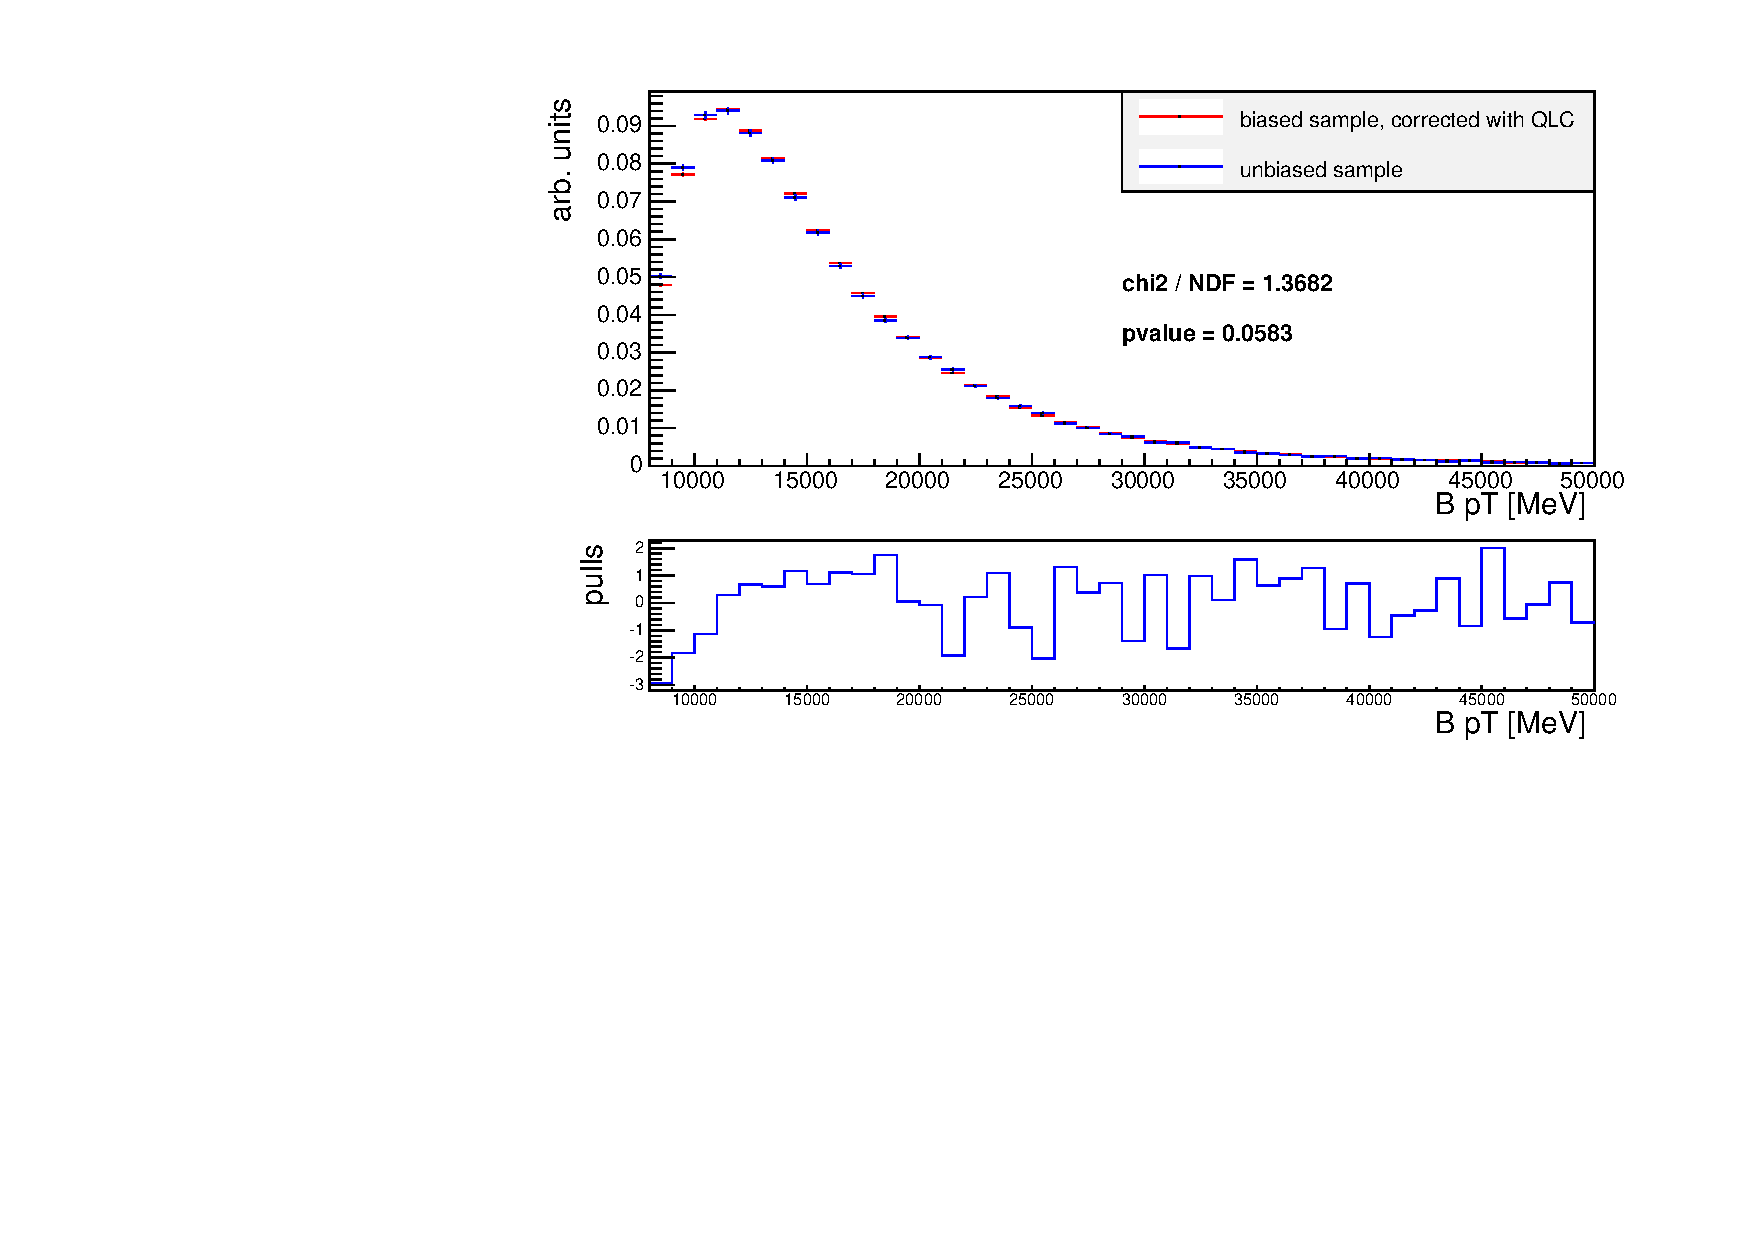
\includegraphics[width=15cm]{figures/InternalNote_MCTuning/oneSample_unbiasedVsQuarkBiasedComparison_pt.pdf}
%  \caption{Plots show the comparison of the $\eta_B$ (first plot) and $pT_B$ (second plot) QLC corrected quark biased distribution and the unbiased disttibution. In order to avoid correlations between the distributions, QLC have been calculated using odd numbered events from the unbiased sample and the QLC corrected quark biased distributions are compared with even numbered unbiased events.}
%  \label{fig:BpQLCapplied_oneSample}
%\end{figure}
%As a cross-check QLC calculated using odd events from the $B^+ \to J/\psi K^+$ unbiased MC have been applied to the quark biased sample and the result has been compared to the distribution of the even unbiased events \ref{fig:BpQLCapplied_oneSample}. The B meson $\eta$ distribution shows good agreement, while the pT distribution shows an inconsistency at low pT. The same effect is visible swapping odd and even unbiased events.\\
%The source of this discrepancy is due to the $\hat{pT}$ cut introduced at generator level, figure  \ref{fig:pTHatComparison_unbiasedVsSemiBiased} shows the $\hat{pT}$ distribution of the unbiased sample and the $\hat{pT}$ distribution from a new sample, semi biased, generated with the same cuts as the unbiased sample but with tigther $\hat{pT}$ (7. GeV instead of 5.), the distribution of the unbiased sample has been cut at 7 GeV in order to compare the two distributions, that are clearly not compatible.\\
%\begin{figure}[h]
%  \centering
%  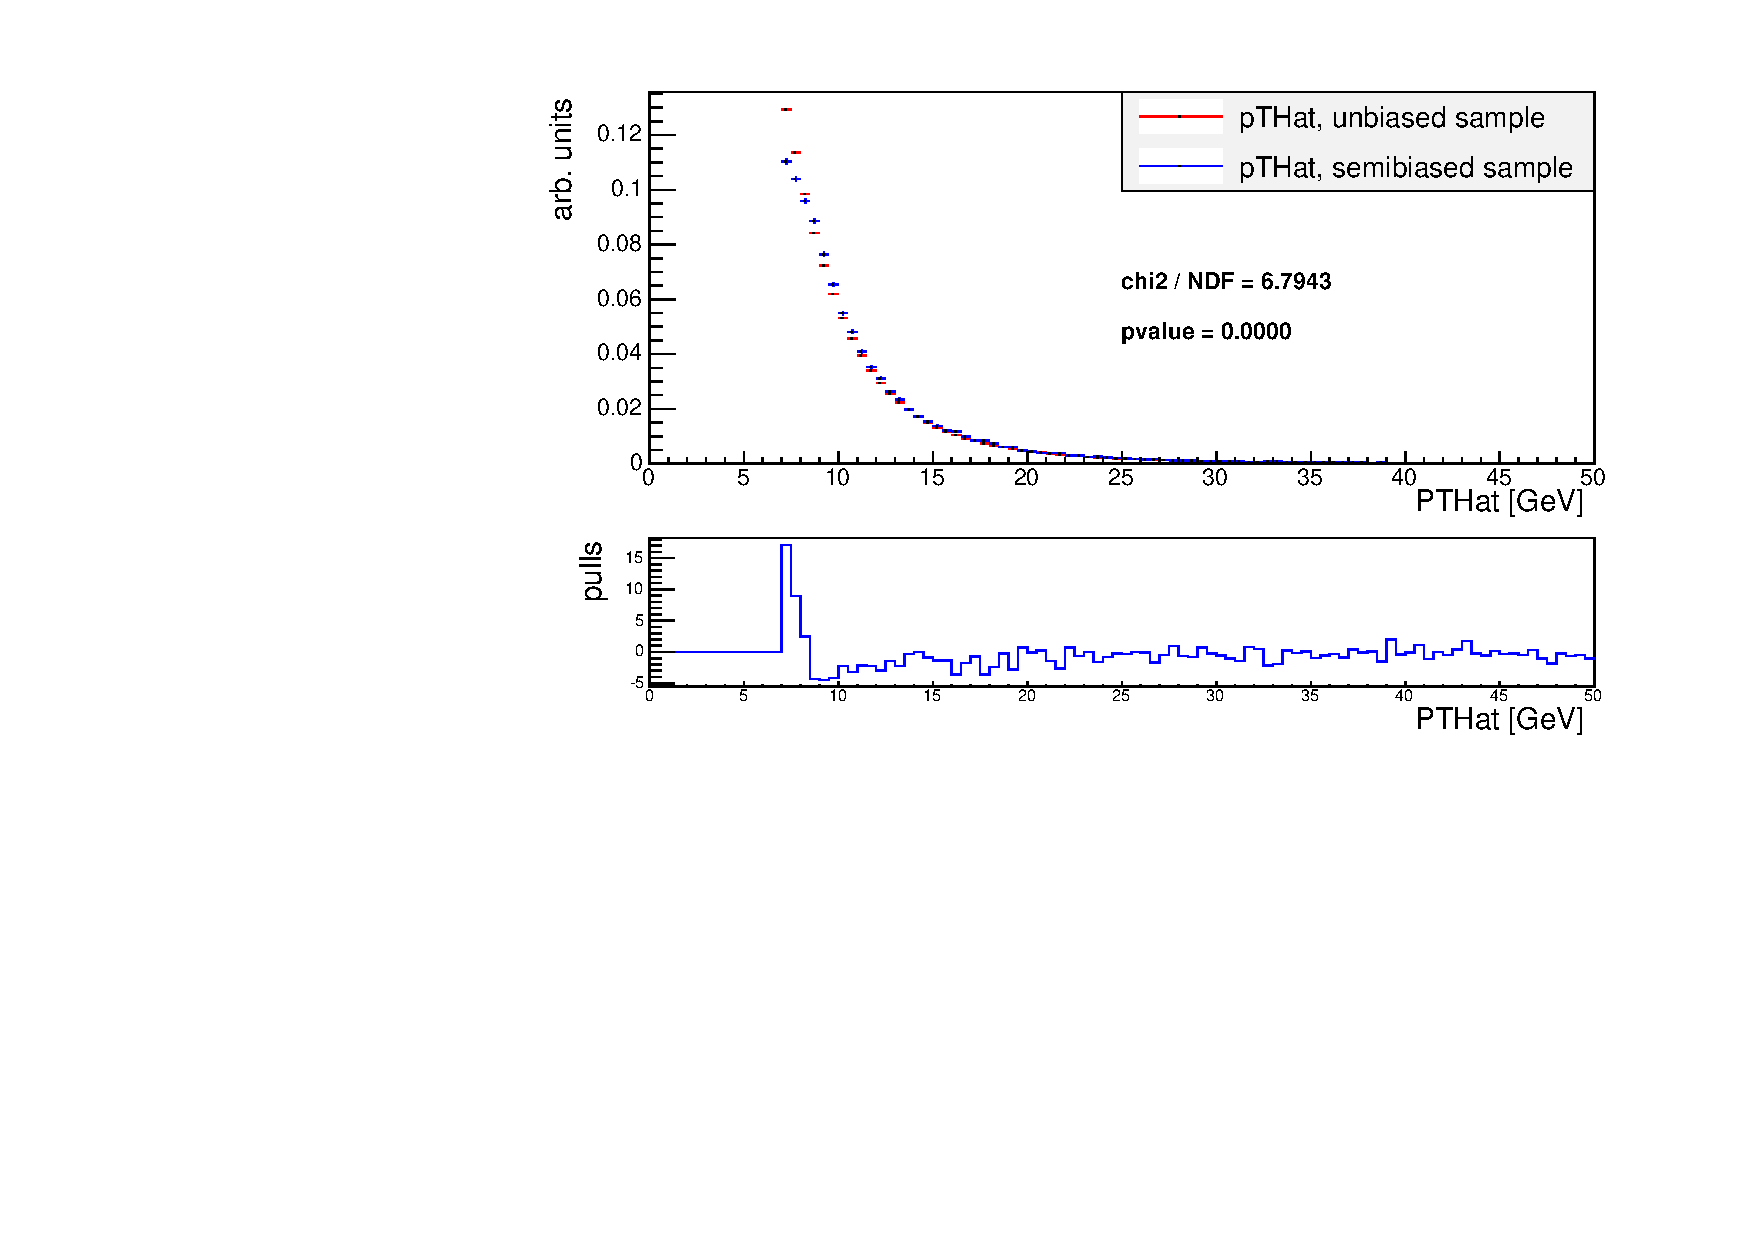
\includegraphics[width=15cm]{figures/InternalNote_MCTuning/PTHatComparison_UnbiasedVsSemiBiased.pdf}
%  \caption{Plot show the comparison of the $\hat{pT}$ distribution from the unbiased sample and the $\hat{pT}$ distribution from a new sample, semi biased, with the same quark-level cuts as the unbiased but with tighter $\hat{pT}$ (7 GeV insted of 5). The unbiased distribution has been cut at 7 GeV in order to compare the two distributions.}
%  \label{fig:pTHatComparison_unbiasedVsSemiBiased}
%\end{figure}
%This is due to a regularisation in the Pythia generation for low $\hat{pT}$ \yel[is the pythia manual in the bib files? not sure]{CITE PYTHIA MANUAL(page14)}; basically the parton-parton cross section becomes too high at low $\hat{pT}$, violating unitarity, this modification smoothly regulates the divergence. 
%QLC calculated using a single unbiased sample are therefore not usable, because they would introduce an additional bias due to this $\hat{pT}$ discrepancy.\\

The computation of the QLC is performed using the unbiased and 
the quark biased samples according to the following formula:
$$   W_{QL} = \nu^{FScuts}_{quarkBiased} \cdot \left(  \frac{\sigma^{Pythia}_{quarkBiased}}{N^{tot}_{quarkBiased}} \right) / \left[ \nu^{FScuts}_{unbiased} \cdot \left( \frac{\sigma^{Pythia}_{unbiased}}{N^{tot}_{unbiased}} \right) \right] $$  
Where $\nu$ is the number of entries in a ($pT_B$, $\eta_B$) from 
the unbiased or quark biased samples after applying the final state 
particle cuts. The term $ \frac{\sigma^{Pythia}}{N^{tot}}$ is used 
to normalise the two MCs to the same integrated 
luminosity: $\sigma^{Pythia}$ is the Pythia generation cross-section 
and $N^{tot}$ is the total number of generated events.\\
The inverse of these weights should be used to weight events 
individually, thus correcting with event-weights the QL cut biases.\\

%%%%%old considerations about the pTHat issue, might go into an appendix (as above)
%Before start calculating the QLC we have to make sure that the unbiased 
%sample we have is not affected by the $\hat{pT}$ bias. Figure 
%\ref{fig:pTHatComparison_unbiasedVsSuperUnbiased} shows the comparison 
%of the $\hat{pT}$ distribution from the unbiased sample and a new sample 
%with the same quark-level cuts as the unbiased but with looser 
%$\hat{pT}$ (3 GeV insted of 5), the distribution of the new sample has 
%been cut at 5 GeV in order to compare the two distributions. We are 
%interested in not having the bias in the parameter space used in the 
%analysis, therefore the quark-level cuts, final state cuts and B 
%fiducial volume cuts ($pT_B$ > 8 GeV and  $|\eta_B|$ < 2.5 ) are applied. 
%The two distributions look compatible, therefore we can use the unbiased sample for the QLC calculation.\\
%\begin{figure}[h]
%  \centering
%  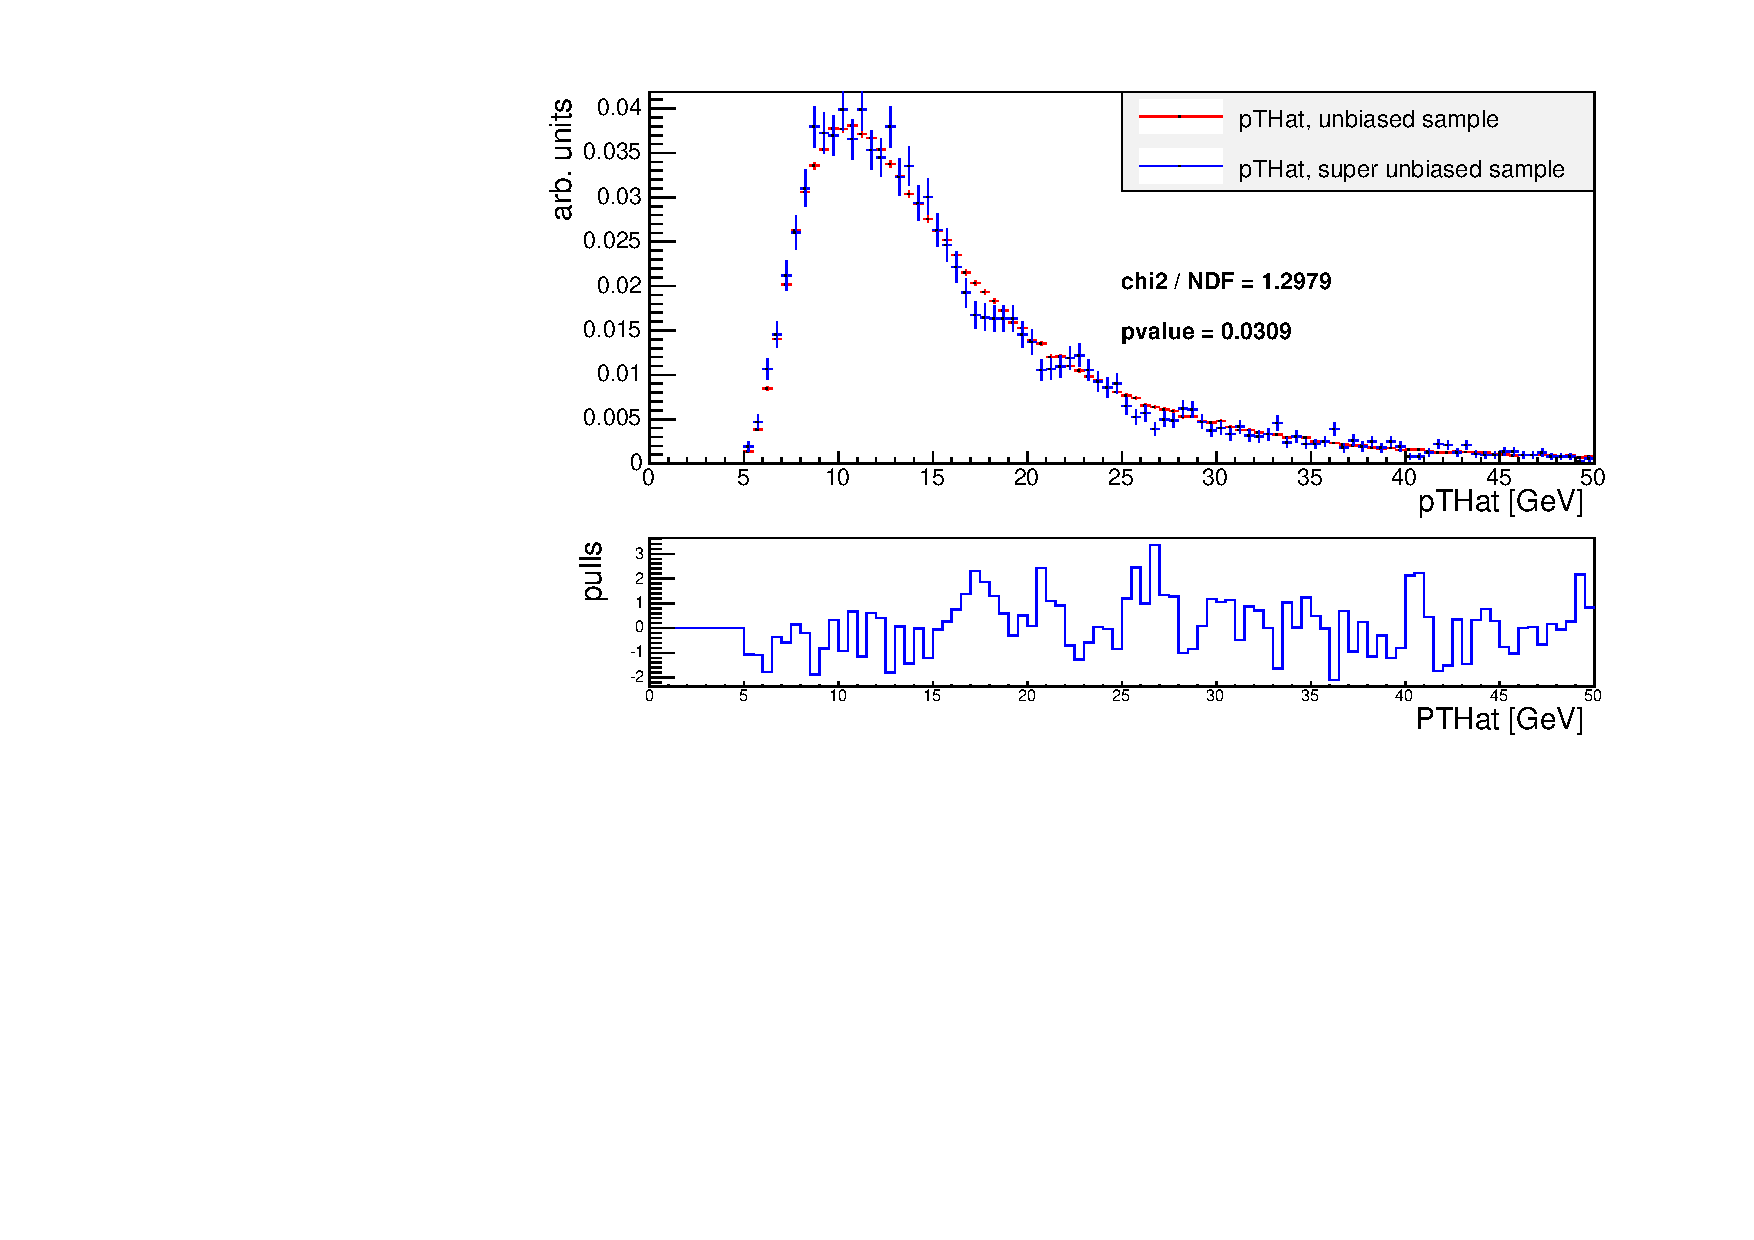
\includegraphics[width=15cm]{figures/InternalNote_MCTuning/pTHatComparison_unbiasedVsSUperUnbiased.pdf}
%  \caption{Plot show the comparison of the $\hat{pT}$ distribution from the unbiased sample and the $\hat{pT}$ distribution from a new sample, super unbiased, with the same quark-level cuts as the unbiased but with looser $\hat{pT}$ (3 GeV insted of 5). The super unbiased distribution has been cut at 5 GeV in order to compare the two distributions. Quark-level cuts, final state cuts and B fiducial volume cuts ($pT_B$ > 8 GeV and  $|\eta_B|$ < 2.5 ) are applied to both distributions.}
%  \label{fig:pTHatComparison_unbiasedVsSuperUnbiased}
%\end{figure}

Figure~\ref{fig:allQLC}  \yel[B+ QLC ready, BsMuMu and BsJpsiPhi QLC still work in progress]{show the QLC calculated for $B^+$, $B_s \rightarrow \mu \mu$, and $B_s J/\psi \phi$  and their uncertainty}.
This computation of the QLC has been cross-check applying 
QLC calculated using odd events, from both the quark biased and 
unbiased samples, to the even events of the quark biased sample. 
The resulting distributions have been compared to unbiased 
distributions obtained using only even events. 
%The inconsistency at low pT has now disappeared, 
Figure \ref{fig:BpQLCapplied_twoSample} 
shows the checks performed on the $B^+$ sample.
\begin{figure}[h]
  \centering
  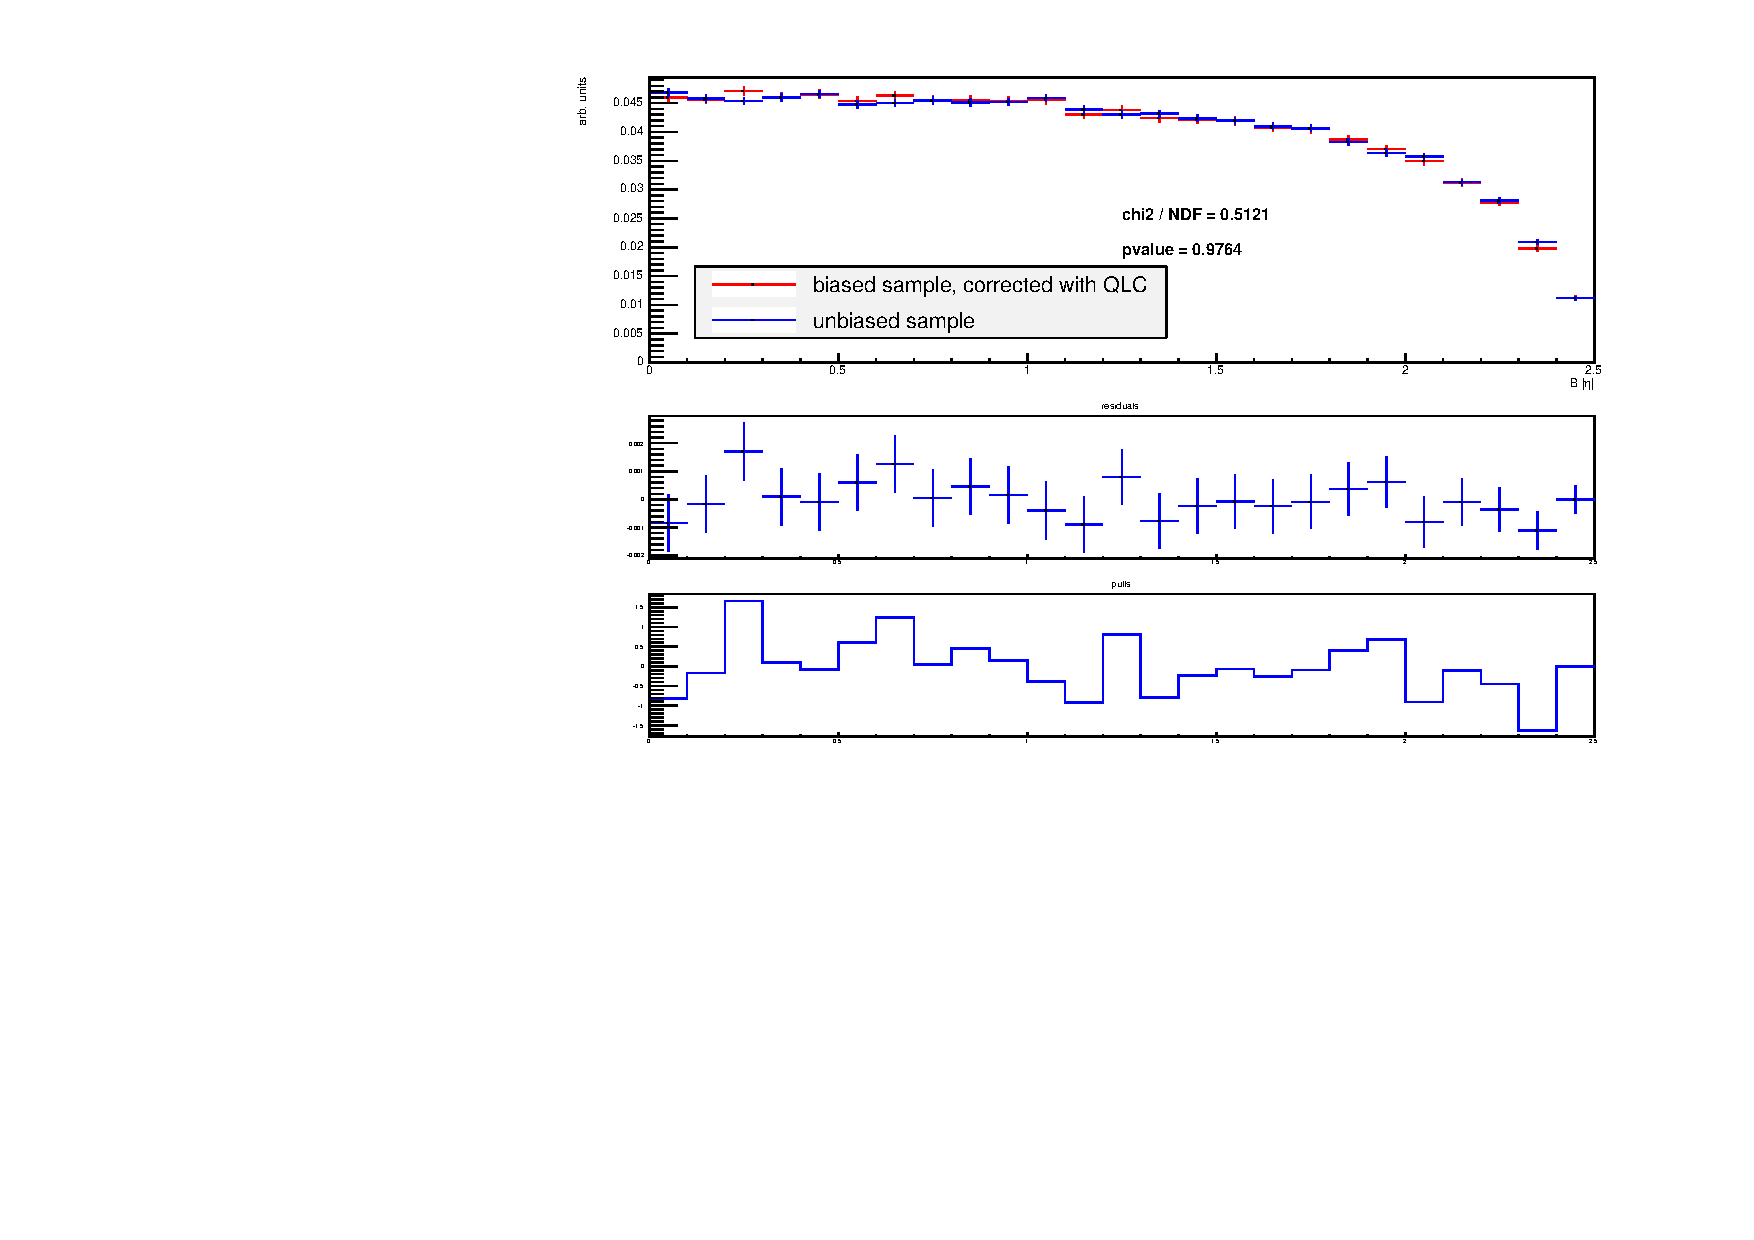
\includegraphics[width=15cm]{figures/InternalNote_MCTuning/twoSampleApproachApplication_etacomparison.pdf}\\
  \vspace{0.5cm}
  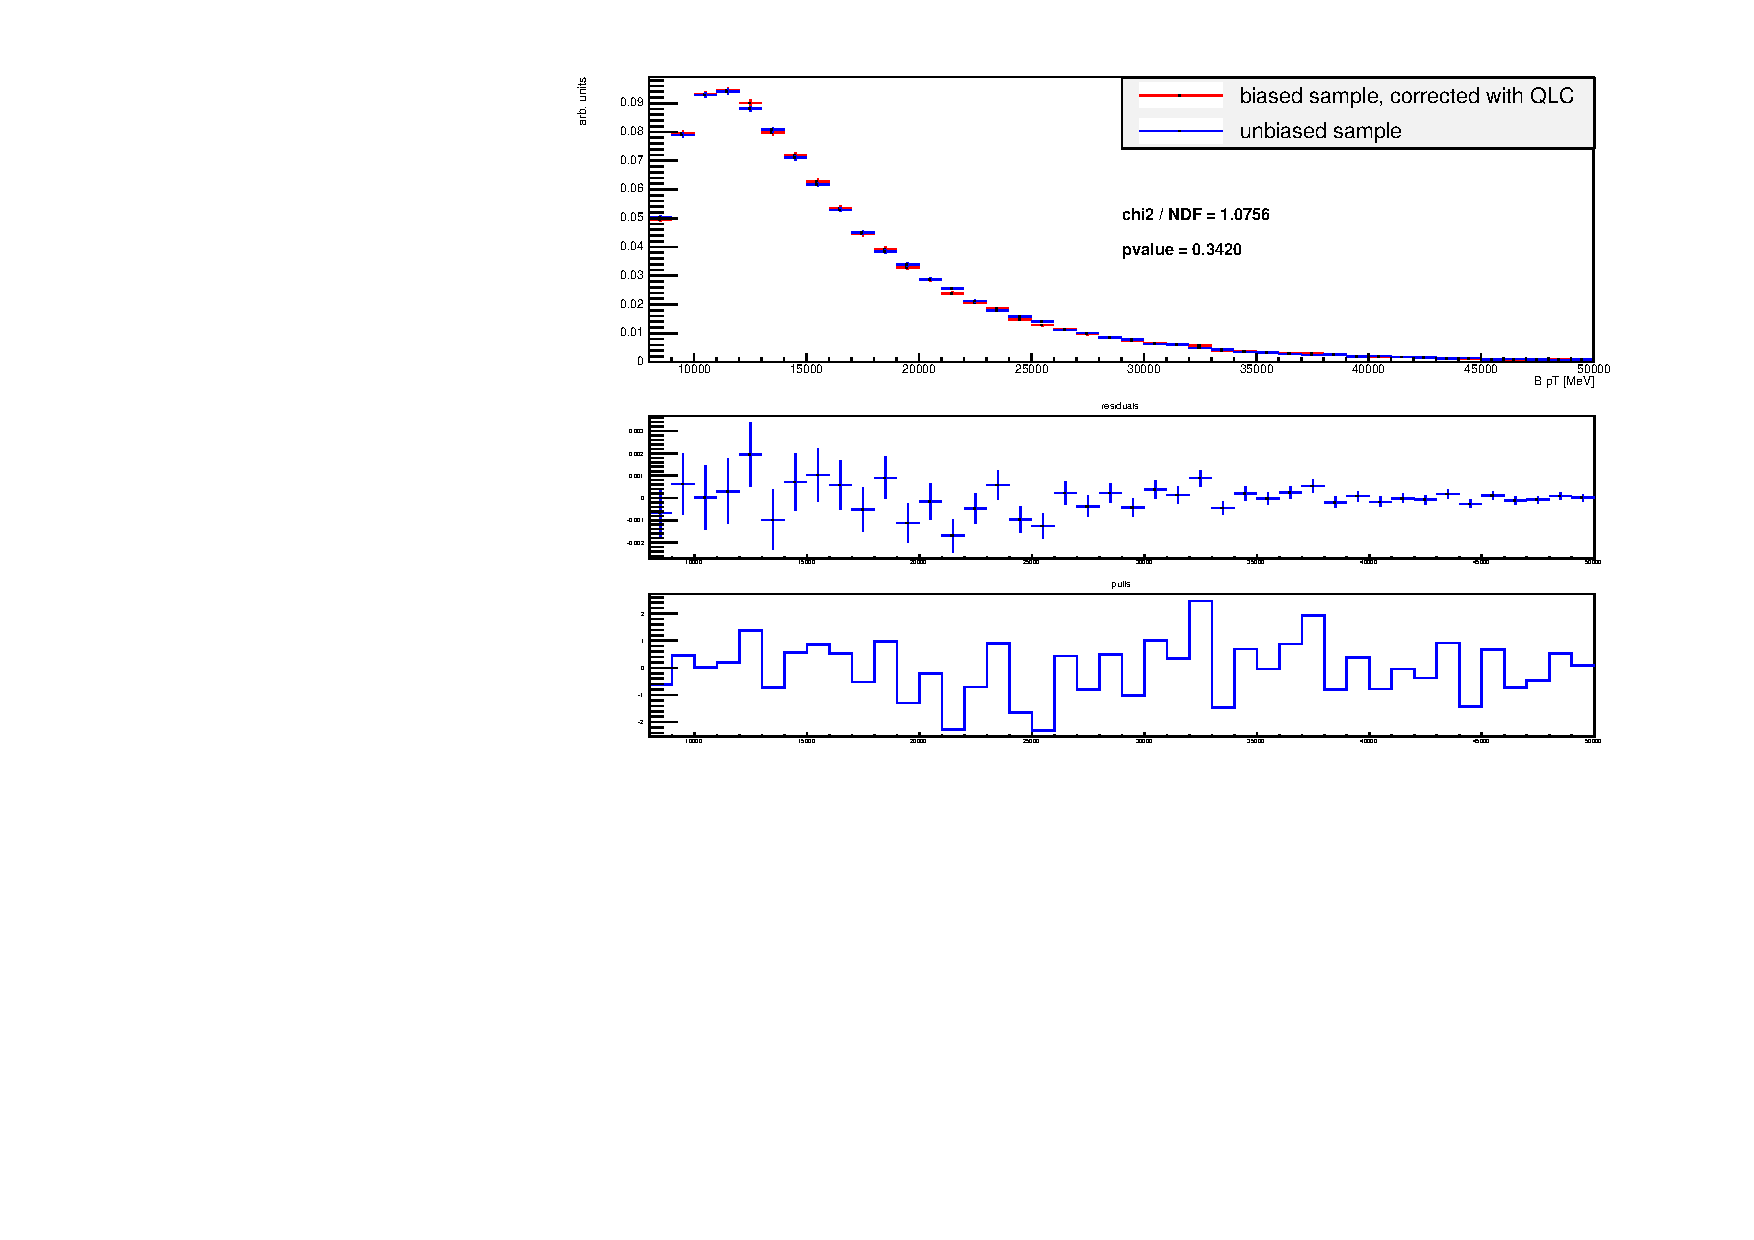
\includegraphics[width=15cm]{figures/InternalNote_MCTuning/twoSampleApproachApplication_pTcomparison.pdf}
  \caption{Plots show the comparison of the $\eta_B$ (first plot) and $pT_B$ (second plot) QLC corrected quark biased distribution using the two samples approach QLC and the unbiased distribution. In order to avoid correlations between the distributions, QLC have been calculated using odd numbered events from the unbiased and quarkBiased samples, and the remaining events in the two samples have been weighted and used for the comparison.}
  \label{fig:BpQLCapplied_twoSample}
\end{figure}











\subsection{Data Driven Weights}
\label{sec:ddw}

The Data Driven Weights (DDW) have been evaluated in a similar way as it 
has been done in~\cite{bsmumuv2} and ~\cite{Alpigiani:1756291}.\footnote
{Due to the limited statistics of the $B^+$ data sample, 
the DDW corrections are not computed in a two-dimensional
grid of the variables $p_T$ and $|y|$, but are extracted with the one-dimensional times %$\times$
one-dimensional procedure described in the text. 
This approach was already used in the analyses~\cite{bsmumuv2} based on 
the 4.7~fb$^{-1}$ sample of data collected in 2011 and~\cite{Alpigiani:1756291} based on the
full Run1 sample.
The validity of the approach is tested by the stability of the recursive procedure,
and fundamentally it works because the production cross-section depends strongly
on $p_T$, but much less on $|y|$, with small correlation
between the two variables. The systematic deviation in the computation of the
average acceptance times %$\times$ 
efficiency due to the method chosen for this analysis
rather than a true two-dimensional computation of the DDW has been estimated
to be at the level of \yel[still work in progress]{.......}
}

The DDW for the MC signal samples are determined with an iterative method,
by comparing sideband-subtracted $B^\pm\to J/\psi K^\pm$ odd-numbered
events with MC events, after the latter are corrected with the $W_\mathrm {QLC}$ weights.\footnote
%
%
{The extraction followed similar lines used in \cite{bsmumuv2} and ~\cite{Alpigiani:1756291}.  
The \Bp yeld was extracted in \pt intervals and alternatively, in $|\eta|$ intervals.
The event selection followed the same line discussed in the following sections of this note, with the addition of 
an additional cut $L_{xy}>0.3$~mm on the transverse separation between primary and secondary vertex, and
without applying the multivariate selection against combinatorial background. The signal is described with
two Gaussians with equal mean; the continuum background is described by an exponential; 
the background due to partially reconstructed decays ($B$ to $J/\psi\, X$, with m($J/\psi \, h^+<5.200$~GeV)  
is described with an error function.
All shape and amplitude parameters are extracted form the fit, and the uncertainty in the signal yield is dominated 
statistical errors. }

We derive two sets of weights, in $\pt$ and $|\eta|$ of the $B$ meson,
determined by the ratio of the normalised $\pt$ and $|\eta|$ spectra
in data and MC.
The final weights that are going to be used are therefore
\begin{equation}
W_\mathrm {DD}\left(\pt,|\eta|\right)=w\left(\pt\right)\cdot w\left(\eta\right)\label{for:ddw}
\end{equation}
where $w={\nu^{data}}/({\nu^{MC}}\times W_\mathrm {QLC})$ and $\nu$ is the normalised
number of entries in either the data or MC histograms for $\pt$ or $\eta$.
\yel[calculaton of DDW underway]{These weights are then used as per-event weights on the MC events, and the
procedure is iterated until these weights stabilise. The stability of the
weights can be seen from the convergence of the second iteration
and it is shown in Figure .....}


%\begin{figure} [!htp]
%  \begin{center}
%  \includegraphics[width=0.88\textwidth ]{eps/glc/ddwCombo_2012_MC2Weighted_withQLC.eps}
%  \caption{
%  {\it Top\/} :DDW extracted for $B^\pm \to J/\psi K^\pm$ as function of $\pt$ ({\it left}) and $\eta$ ({\it right}) of the $B$ meson. 
%    {\it Bottom\/}: the same as above showing the separately the result of the first iteration (blue points) 
%    and the small additional correction (red points) from the second iteration.
%    }
%  \label{fig:ddwBplus}
%  \end{center}
%\end{figure}




%Events from \Bs \ decays into $J/\psi\, \phi \to \mu^+\mu^-\K^+\K^-$ can be studied
%and compared to \Bp \ decays to $J/\psi \,K^+$.  In particular, DDW can be extracted in the
%$J/\psi\, \phi $ channel and compared the standard ones from  $J/\psi K^+$.
%This is shown in Figure~\ref{fig:ddwJPsiPhi}.\footnote
%{Here the data points for \Bp \ were obtained without reweighting the MC sample
%according to the pre-L2StarB and L2StarB trigger configuration and without applying data-driven
%corrections to the trigger efficiency, causing a minor
%difference from the plot in Figure~\ref{fig:ddwBplus}. The treatment was consistent
%between the two channels, and the comparison is not significantly affected.}
%The two sets of weights agrees well within the the statistical error, confirming
%that the relative yield of \Bs \ and \Bp does not to depend significantly on \pt \
%and \eta ~\cite{Aaij:2013qqa, lhcbfsfu14}, and providing a consistency check on our
%procedures. Furthermore, the comparison supports the assumption of using DDW derived
%from \Bp \ also  for the \Bs \ channel. 
%\begin{figure} [!htp]
%  \begin{center}
%  \includegraphics[width=0.65\textwidth ]{eps/glc/compare_JpsiPhi_JpsiKplus_MC1Weighted.eps}
%  \caption{
%  Comparison of DDW for $\Bp \to J/\psi K^+$ (blue points) and $\Bs \to J/\psi \phi$ (red points).}  
%  \label{fig:ddwJPsiPhi}
%  \end{center}
%\end{figure}


\clearpage
